\pgfplotsset{compat=1.16}
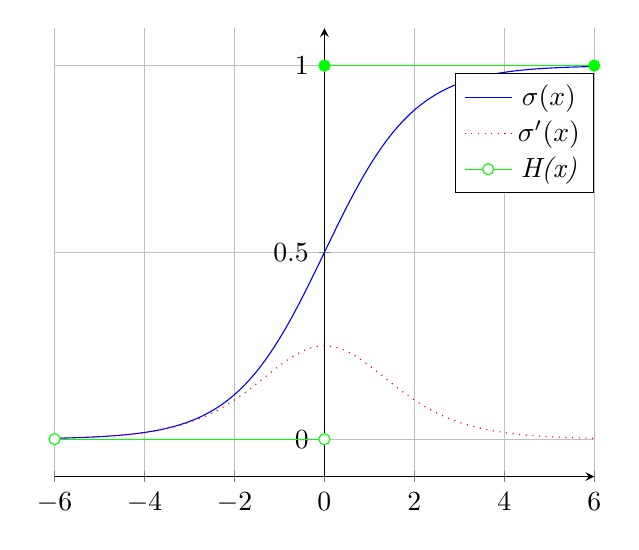
\begin{tikzpicture}[declare function={sigma(\x)=1/(1+exp(-\x));
sigmap(\x)=sigma(\x)*(1-sigma(\x));}]
\begin{axis}%
[
    grid=major,     
    xmin=-6,
    xmax=6,
    axis x line=bottom,
    ytick={0,.5,1},
    ymax=1.1,
    ymin=-0.1,
    axis y line=middle,
    samples=100,
    domain=-6:6,
    legend style={at={(1,0.9)}}     
]
    \addplot[blue,mark=none]   (x,{sigma(x)});
    \addplot[red,dotted,mark=none]   (x,{sigmap(x)});
    % \addplot[green,mark=none] {(-6, 0), (-0.2, 0), (0.2, 1), (6, 1)};
    \addplot[green, mark=*, mark options={fill=white}, samples at={-6, 0}] {0};
    \addplot[green, mark=*, samples at={0, 6}] {1};
    \legend{$\sigma(x)$,$\sigma'(x)$, $\textit{H(x)}$}
\end{axis}
\end{tikzpicture}
